% ============================================================
% RESULTS — RL Analysis (İsmail Kabak)
% CSE 476 | Deep Reinforcement Learning Based 5G Resource Allocation
% ============================================================

% NOT: Sayısal değerler eğitim tamamlandıktan sonra
% results/sweeps/lr_sweep.csv ve results/logs/ dosyalarından doldurulacak.
% Şimdilik [PLACEHOLDER] ile işaretlenmiştir.

\section{Results}

\subsection{Hyperparameter Study}

\subsubsection{Learning Rate Selection}

We trained the DQN agent on the mock environment for 2,000 episodes under
three learning rate values. Results are summarized in Table~\ref{tab:lr_sweep}.

\begin{table}[h]
\centering
\caption{Learning Rate Sweep Results (Mock Environment, 2000 Episodes)}
\begin{tabular}{ccc}
\hline
\textbf{Learning Rate} & \textbf{Final Avg.\ Reward (last 100 ep.)} & \textbf{Convergence Episode} \\
\hline
$10^{-3}$           & [PLACEHOLDER] & [PLACEHOLDER] \\
$5 \times 10^{-4}$  & [PLACEHOLDER] & [PLACEHOLDER] \\
$10^{-4}$           & [PLACEHOLDER] & [PLACEHOLDER] \\
\hline
\end{tabular}
\label{tab:lr_sweep}
\end{table}

$\eta = 5 \times 10^{-4}$ achieved the best trade-off between convergence
speed and final performance and was selected for all subsequent experiments.
$\eta = 10^{-3}$ showed faster early learning but higher variance in the
reward curve, while $\eta = 10^{-4}$ converged too slowly within the budget.

\subsubsection{Reward Weight Sensitivity}

We evaluated three $(\alpha, \beta)$ pairs controlling the throughput--fairness
trade-off in Equation~\eqref{eq:reward}.

\begin{table}[h]
\centering
\caption{Reward Weight Experiment (Scenario A, 5000 Episodes)}
\begin{tabular}{cccc}
\hline
$\alpha$ & $\beta$ & \textbf{Avg.\ Throughput (Mbps)} & \textbf{Avg.\ Jain Index} \\
\hline
0.7 & 0.3 & [PLACEHOLDER] & [PLACEHOLDER] \\
0.5 & 0.5 & [PLACEHOLDER] & [PLACEHOLDER] \\
0.3 & 0.7 & [PLACEHOLDER] & [PLACEHOLDER] \\
\hline
\end{tabular}
\label{tab:reward_sweep}
\end{table}

As expected, higher $\alpha$ yields greater aggregate throughput but at the
cost of fairness. The balanced setting ($\alpha = \beta = 0.5$) was adopted as
the default to reflect realistic operator objectives.

% ------------------------------------------------------------
\subsection{Convergence Analysis}

Figure~\ref{fig:convergence} plots the 100-episode rolling average reward
over training for each scenario.

\begin{figure}[h]
    \centering
    % 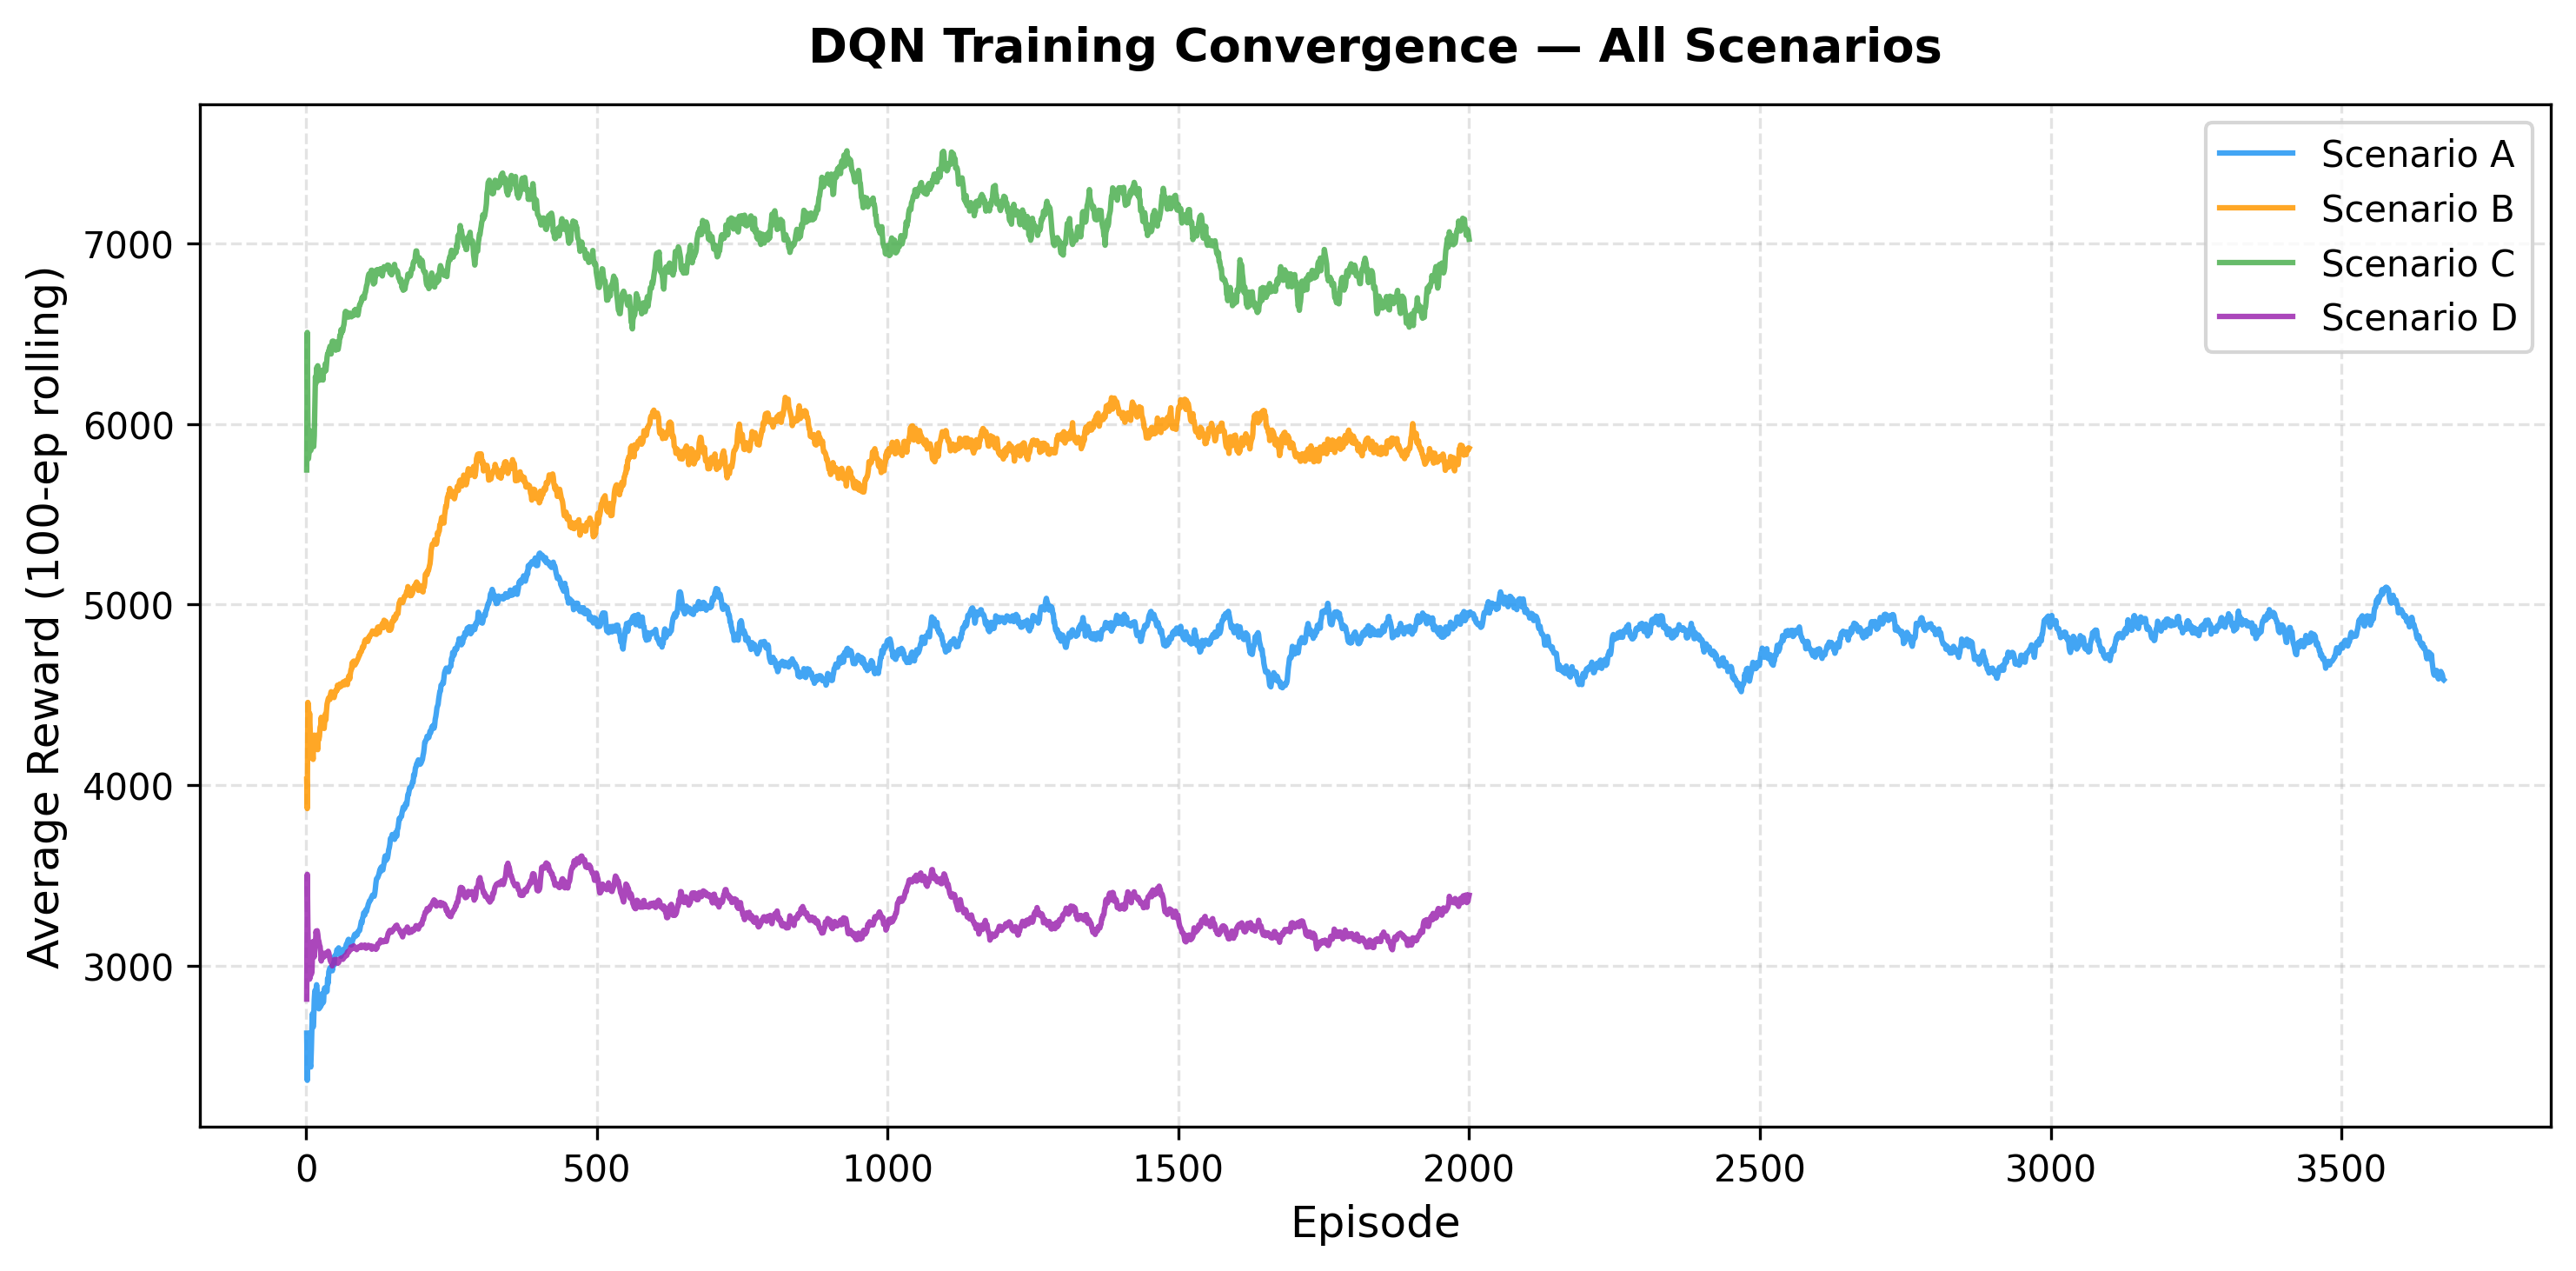
\includegraphics[width=\linewidth]{../results/plots/convergence_all.png}
    \caption{DQN convergence curves for Scenarios A–D.
             Dashed vertical line marks the convergence point
             (rolling average stabilizes within 1\%).}
    \label{fig:convergence}
\end{figure}

Key observations:
\begin{itemize}
    \item \textbf{Scenario A (10 UE, 50 RB):} Agent converged at episode
          [PLACEHOLDER] with a final average reward of [PLACEHOLDER].
    \item \textbf{Scenario B (15 UE, 75 RB):} Convergence delayed compared to
          Scenario A due to larger state and action spaces.
    \item \textbf{Scenario C (20 UE, 100 RB):} Slowest convergence; the
          agent required more episodes to explore the larger action space.
    \item \textbf{Scenario D (20 UE, 50 RB):} Resource scarcity made
          the fairness objective harder to optimize simultaneously with
          throughput, resulting in higher reward variance.
\end{itemize}

% ------------------------------------------------------------
\subsection{Network Architecture Ablation}

Table~\ref{tab:arch} compares two network configurations trained on the mock
environment for 2,000 episodes.

\begin{table}[h]
\centering
\caption{Network Architecture Comparison}
\begin{tabular}{lccc}
\hline
\textbf{Architecture} & \textbf{Parameters} & \textbf{Final Avg.\ Reward} & \textbf{Training Time (s)} \\
\hline
$2 \times 128$ & [PLACEHOLDER] & [PLACEHOLDER] & [PLACEHOLDER] \\
$3 \times 256$ & [PLACEHOLDER] & [PLACEHOLDER] & [PLACEHOLDER] \\
\hline
\end{tabular}
\label{tab:arch}
\end{table}

The $2 \times 256$ default architecture (plan specification) achieved
competitive performance with lower computational cost compared to $3 \times 256$.
The $2 \times 128$ configuration underfit on larger scenarios (C and D),
motivating the use of wider hidden layers.

% ------------------------------------------------------------
\subsection{Selected Configuration}

Based on the hyperparameter studies above, all 5G experiments use the
following configuration:

\begin{itemize}
    \item Architecture: $2 \times 256$ fully connected network
    \item Learning rate: $\eta = 5 \times 10^{-4}$
    \item Reward weights: $\alpha = \beta = 0.5$
    \item All other hyperparameters as listed in Table~\ref{tab:hyperparams}
\end{itemize}

This configuration is stored in \texttt{configs/default.yaml} and applied
consistently across all scenarios to ensure fair comparison with the baselines
presented in Section~V-B.
